 %\documentclass[12pt,a4paper,oneside]{report}

\documentclass[12pt,a4paper,openright,twoside]{report}
\usepackage[hmarginratio=1:1]{geometry}
\usepackage[italian]{babel}
\usepackage[T1]{fontenc}
\usepackage[utf8]{inputenc}
\usepackage{listings}
\usepackage{upquote}
\usepackage{framed,xcolor,verbatim}
\usepackage{emptypage} %removes header and footers from empty pages
\definecolor{lightgray}{rgb}{0.95, 0.95, 0.95}
\definecolor{darkgray}{rgb}{0.4, 0.4, 0.4}
\definecolor{editorGray}{rgb}{0.98, 0.98, 0.98}
\definecolor{editorOcher}{HTML}{FF7F00}
\definecolor{green}{HTML}{0D9E0D}
\definecolor{orange}{HTML}{CF7B2F}
\definecolor{red}{HTML}{D53235}
\definecolor{olive}{rgb}{0.17,0.59,0.20}
\definecolor{brown}{rgb}{0.69,0.31,0.31}
\definecolor{purple}{HTML}{BC5298}
\definecolor{lightblue}{rgb}{0.1,0.57,0.7}
\definecolor{lightred}{rgb}{1,0.4,0.5}

% JavaScriptnpm sta
\lstdefinelanguage{JavaScript}{
  keywords={break, case, catch, continue, debugger, default, delete, do, else, false, finally, for, function, if, in, instanceof, new, null, return, switch, true, try, typeof, var, void, while, with, const, let},
  ndkeywords={class, export, boolean, throw, implements, import, this},
  morecomment=[s]{/*}{*/},
  morecomment=[l]//,
  morestring=[b]",
  morestring=[b]`,
  morestring=[b]',
  % Code design
  identifierstyle=\color{black},
  keywordstyle=\color{purple}\bfseries,
  ndkeywordstyle=\color{red}\bfseries,
  stringstyle=\color{green}\ttfamily,
  commentstyle=\color{darkgray}\ttfamily,
}
\lstset{
   language=JavaScript,
   backgroundcolor=\color{editorGray},
   extendedchars=true,
   basicstyle=\footnotesize\ttfamily,
   showstringspaces=false,
   showspaces=false,
   numbers=left,
   numberstyle=\tiny,
   numbersep=9pt,
   frameround=tttt,
   frame=single,
   tabsize=3,
   breaklines=true,
   showtabs=false,
   captionpos=b
}

%\usepackage[latin1]{inputenc}
\usepackage{indentfirst}
\usepackage{fancyhdr}
\usepackage{natbib}
\usepackage{newlfont}
\usepackage{hyperref}
\usepackage{url}

\definecolor{shadecolor}{rgb}{.9, .9, .9}

\newenvironment{code}%
   {\snugshade\verbatim}%
   {\endverbatim\endsnugshade}

\usepackage{graphicx}
\usepackage{svg}
\usepackage{afterpage}

\newcommand\blankpage{%
    \null
    \thispagestyle{empty}%
    \addtocounter{page}{-1}%
    \newpage}

%\usepackage{showkeys} serve per mostrare le etichette, va tolta per la versione definitiva;
%\linespread{1.3}
\oddsidemargin=0pt
\textwidth=450pt
%\hyphenation{} %serve per la sillabazione
\hypersetup{
    colorlinks,
    citecolor=black,
    filecolor=black,
    linkcolor=black,
    urlcolor=black
}

\setlength{\parindent}{0pt}


%\pagestyle{fancy}\addtolength{\headwidth}{20pt}
\renewcommand{\chaptermark}[1]{\markboth{\thechapter.\ #1}{}}
\renewcommand{\sectionmark}[1]{\markright{\thesection \ #1}{}}
%\rhead[\fancyplain{}{\bfseries\leftmark}]{\fancyplain{}{\bfseries\thepage}}
\cfoot{}

\begin{document}

%%%%%%%%%%%%%%%%%%%%%%%%%%%%%%%%%%%%%%%%%%%%%%%%%%%%%%%%%%%%%%%%%%%%%%%%%%%
						% Frontespizio
%%%%%%%%%%%%%%%%%%%%%%%%%%%%%%%%%%%%%%%%%%%%%%%%%%%%%%%%%%%%%%%%%%%%%%%%%%%

\begin{titlepage}
\begin{center}
{{\Large{\textsc{Alma Mater Studiorum $\cdot$ Universit\`a di
Bologna}}}} \rule[0.1cm]{15.8cm}{0.1mm}
\rule[0.5cm]{15.8cm}{0.6mm}
{\small{\bf SCUOLA DI SCIENZE\\
Corso di Laurea in Informatica }}
\end{center}
\vspace{40mm}
\begin{center}
{\LARGE{\bf Resource-centric push model}}\\
\vspace{3mm}
{\LARGE{\bf over WebSockets}}\\
\end{center}
\vspace{40mm}
\par
\noindent
\begin{minipage}[t]{0.47\textwidth}
{\large{\bf Relatore:\\
Chiar.mo Prof.\\
Fabio Vitali}}
\end{minipage}
\hfill
\begin{minipage}[t]{0.47\textwidth}\raggedleft
{\large{\bf Presentata da:\\
Filippo Vigani}}
\end{minipage}
\vspace{30mm}
\begin{center}
{\large{\bf Sessione I\\%inserire il numero della sessione in cui ci si laurea
Anno Accademico 2018-2019}}%inserire l'anno accademico a cui si è iscritti
\end{center}
\end{titlepage}
\newgeometry{margin=1.5in}
\pagenumbering{roman}

%%%%%%%%%%%%%%%%%%%%%%%%%%%%%%%%%%%%%%%%%%%%%%%%%%%%%%%%%%%%%%%%%%%%%%%%%%%
							% Dedica
%%%%%%%%%%%%%%%%%%%%%%%%%%%%%%%%%%%%%%%%%%%%%%%%%%%%%%%%%%%%%%%%%%%%%%%%%%%

\cleardoublepage

\cleardoublepage
\thispagestyle{empty}
\vspace*{\stretch{1}}
\large                                  %aumenta la grandezza del carattere a 14pt
\begin{flushright}
\em
\itshape

\end{flushright}
\vspace{\stretch{2}}
\cleardoublepage


\afterpage{\blankpage}

\linespread{1.3}
%\textwidth=345.0pt

%%%%%%%%%%%%%%%%%%%%%%%%%%%%%%%%%%%%%%%%%%%%%%%%%%%%%%%%%%%%%%%%%%%%%%%%%%%
							% Indice
%%%%%%%%%%%%%%%%%%%%%%%%%%%%%%%%%%%%%%%%%%%%%%%%%%%%%%%%%%%%%%%%%%%%%%%%%%%
\pagenumbering{roman}\normalsize
\clearpage{\pagestyle{empty}\cleardoublepage}
\tableofcontents
%\rhead[\fancyplain{}{\bfseries\leftmark}]{\fancyplain{}{\bfseries\thepage}}
%\lhead[\fancyplain{}{\bfseries\thepage}]{\fancyplain{}{\bfseries INDICE}}

\listoffigures
\addcontentsline{toc}{chapter}{Elenco delle figure}

%%%%%%%%%%%%%%%%%%%%%%%%%%%%%%%%%%%%%%%%%%%%%%%%%%%%%%%%%%%%%%%%%%%%%%%%%%%
							% Introduzione
%%%%%%%%%%%%%%%%%%%%%%%%%%%%%%%%%%%%%%%%%%%%%%%%%%%%%%%%%%%%%%%%%%%%%%%%%%%

\chapter*{Introduzione}
%\rhead[\fancyplain{}{\bfseries INTRODUZIONE}]{\fancyplain{}{\bfseries\thepage}}
%\lhead[\fancyplain{}{\bfseries\thepage}]{\fancyplain{}{\bfseries INTRODUZIONE}}
\addcontentsline{toc}{chapter}{Introduzione}
Quando si sviluppa un’applicazione web, si deve considerare che meccanismo di data delivery utilizzare. Spesso si vuole sviluppare un’applicazione che lavori con dati in tempo reale: può essere una dashboard con l’andamento di un mercato azionario, o una console di un servizio backend su cui lavorano più utenti, o ancora un semplice calendario condiviso per la gestione di appuntamenti.

\bigskip

Per molto tempo l’unica modalità per reperire i dati da un web browser è stata tramite client pull, ovvero il client si occupa di richiedere una risorsa, e richiedere se la risorsa stessa sia stata modificata.

\bigskip

Con l’implementazione dei websocket nella maggior parte dei browser, la situazione cambia. Si apre la possibilità di ricevere dati tramite server push, senza dover periodicamente richiedere una risorsa, ma lasciando al server l’onere di notificare i client dell’avvenuta modifica della risorsa.

\bigskip

Tuttavia i websocket rimangono un’implementazione di basso livello, e lavorarci su applicazioni di alto livello, dove l’architettura e la separation of concerns è un punto focale, risulta complesso.

\bigskip

La soluzione proposta permette in modo semplice ed intuitivo di rimanere in ascolto di una risorsa come se fosse un endpoint REST, e ogni qualvolta questa risorsa venga aggiornata, essere notificati del nuovo contenuto, senza doversi preoccupare di una gestione efficiente delle risorse.

%%%%%%%%%%%%%%%%%%%%%%%%%%%%%%%%%%%%%%%%%%%%%%%%%%%%%%%%%%%%%%%%%%%%%%%%%%%
							% Background
%%%%%%%%%%%%%%%%%%%%%%%%%%%%%%%%%%%%%%%%%%%%%%%%%%%%%%%%%%%%%%%%%%%%%%%%%%%
\chapter{Background}
\pagestyle{fancy}
\lhead[\rmfamily\thepage]{\fancyplain{}{\itshape\nouppercase\rightmark}} % respectively left page inner and right page inner 
\rhead[\fancyplain{}{\itshape\nouppercase\leftmark}]{\rmfamily\thepage} % respectively left page outer and right page outer 
%\rhead[\fancyplain{}{\bfseries\thepage}]{\fancyplain{}{\bfseries\rightmark}}
%\lhead[\fancyplain{}{\bfseries\thepage}]{\fancyplain{}{\bfseries\leftmark}}
\pagenumbering{arabic}

Nello sviluppo di applicazioni web moderne spesso si ha la necessità di aggiornare parti dell’interfaccia in modo che rispecchino delle risorse non presenti localmente in tempo reale. Si pensi per esempio ad un’applicazione che deve visualizzare i dati dello stock market, o ad un social network, o ad un calendario per la gestione degli appuntamenti, o ancora ad una semplice dashboard di gestione aziendale. 

\bigskip

In tutti questi casi, poter vedere le modifiche effettuate da terzi sulle stesse risorse in real-time è essenziale o migliora di gran lunga la user experience. Le applicazioni real-time stanno gradualmente dominando l’internet in quanto forniscono un perfetto equilibrio di informazioni, funzionalità, contenuto e interattività che portano ad aumentare lo user engagement.

%%%%%%%%%%%%%%%%%%%%%%%%%
			% Sviluppo app moderne real-time
%%%%%%%%%%%%%%%%%%%%%%%%%
\section{Sviluppo app moderne real-time}\label{sec_appmoderne}

Con applicazioni real-time intendiamo applicazioni che permettano di ricevere e visualizzare degli aggiornamenti che risiedono su un server nel minor tempo possibile. Da una definizione così banale, spuntano in realtà una serie di questioni importanti per quanto concerne sia le tecnologie per implementarle, che le tecniche utilizzate che la gestione delle risorse.

\bigskip

Gli sviluppatori web, fino a qualche anno fa, per ottenere dei risultati simili hanno dovuto sfruttare diverse tecniche che aggirassero le limitazioni dei browser. Infatti l’unico modo di ricevere dati per un browser era quello di inviare una richiesta al server, e ricevere una risposta. Ciò significa che il client non aveva modo di essere notificato in caso la risorsa richiesta venisse modificata.

%%%%%%%%%%%%%%%%%%%%%%%%%
			% Client pull
%%%%%%%%%%%%%%%%%%%%%%%%%
\section{Client pull}\label{sec_clientpull}

Questo stile di comunicazione ove la richiesta è originata dal client e risposta dal server è chiamato \textit{client pull}. Il client pull forma la base per la comunicazione tra un browser e un server tramite il protocollo HTTP, e su di esso si sono costruiti una serie di stili architetturali per fornire interoperabilità tra web services in maniera prestabilita. Per esempio, uno degli stili più utilizzati è REST (REpresentational State Transfer), che stabilisce che i web services devono permettere ad altri sistemi di richiedere l’accesso o la manipolazione di rappresentazioni testuali di risorse web usando un insieme predefinito di operazioni stateless.

\bigskip

Un protocollo stateless prevede che il server non mantenga nessuna informazione riguardante la connessione attiva del client tra una richiesta e l’altra. Non mantenendo alcun tipo di informazione sulla sessione, ne consegue che per verificare se una risorsa è stata aggiornata rispetto a quella salvata da un browser in precedenza, è necessario richiedere la stessa risorsa e compararla con la precedente.

%%%%%%%%%%%%%%%%%%%%%%%%%
		% Polling e long polling
%%%%%%%%%%%%%%%%%%%%%%%%%
\subsection{Polling e long polling}

Una delle tecniche largamente utilizzate per verificare se una risorsa, web o meno, sia stata modificata è appunto richiedere la stessa risorsa a intervalli regolari, e confrontarla con la precedente. Questa tecnica nella letteratura è chiamata polling. Nell’ambito dei web services e di HTTP, si possono distinguere due tipi di polling: Polling semplice e long polling
\begin{description}
\item Nel \textbf{polling semplice} la risorsa viene richiesta periodicamente e il server risponde immediatamente con la risorsa richiesta. Ad un livello più basso, viene aperta una connessione, inviato un messaggio dal client al server contenente la richiesta, inviato un messaggio di risposta dal server al client contenente la risorsa, e la connessione viene chiusa. Successivamente, dopo un periodo di polling prestabilito, si ripete.
Un esempio di utilizzo di polling client side potrebbe essere il seguente:
\lstinputlisting[caption=Client side XHR polling example]{snippets/polling_sample.js}

\begin{figure}[htbp]
\centering

\includegraphics[width=.8\textwidth]{assets/polling.png}
\caption{Polling}
\end{figure}

\item Nel caso del \textbf{long polling}, conosciuto anche come \textit{hanging GET} o \textit{COMET}, invece, il client invia una richiesta ad una risorsa specifica. Il server, invece di rispondere immediatamente, tiene aperta la connessione fintanto che la risorsa non viene aggiornata o finché una soglia di timeout viene superata. Quando sono presenti nuovi dati, il server risponde alla richiesta chiudendo la connessione di conseguenza. Dopodiché il client richiede nuovamente la stessa risorsa e rimane in attesa.
Questo flusso può essere implementato come l'esempio seguente:
\lstinputlisting[caption=Client side XHR long polling example]{snippets/longpolling_sample.js}

\begin{figure}[htbp]
\centering

\includegraphics[width=.8\textwidth]{assets/long_polling.png}
\caption{Long polling}
\end{figure}

A differenza del polling semplice, dove l’implementazione riguarda solo la parte client, e il server espone un semplice endpoint REST, nel long polling il server deve supportare questo tipo di interazione con il client. Infatti, oltre ad esporre un semplice endpoint REST, dovrà esporre un endpoint che si occupa di mantenere il client in attesa, ed inviare la risposta solo una volta che viene aggiornata la risorsa. Inoltre, dovrà gestire lo stato di connessioni multiple, ed implementare strategie per preservare lo stato delle sessioni quando si utilizzano più server e load balancers.

\end{description}

\subsection{Problematiche}
Entrambe le tecniche di polling sono dei workaround dovute alle storiche limitazioni dei browser e di HTTP, e dunque presentano delle problematiche. 
% Consumo di banda e traffico dati
\subsubsection{Consumo di banda e traffico dati}
Poiché il polling richiede ad intervalli regolari la stessa risorsa, spreca traffico dati per passare sia la richiesta della risorsa stessa, che per ricevere il payload effettivo. In particolare per ogni richiesta HTTP, deve essere stabilita una nuova connessione, si deve fare il parsing degli header HTTP, si deve presumibilmente reperire i dati da un database, e infine inviare i dati al client.

% Ritardo
\subsubsection{Ritardo}
Per limitare questo consumo, si cerca di trovare un equilibrio riducendo la frequenza di poll. Ma così facendo, risulta che per ricevere un aggiornamento di una risorsa, il client potrebbe aspettare fino alla durata dell’intervallo di tempo tra una richiesta e la successiva.

% Incoerenza dei dati
\subsubsection{Incoerenza dei dati}
Nel caso del long polling, la risorsa viene inviata presumibilmente appena subisce delle modifiche. Tuttavia nel lasso di tempo che passa tra quando il client riceve una risposta, ed effettua la nuova richiesta da tenere aperta, la risorsa stessa potrebbe essere modificata. In tal caso, il server non ha nessuna connessione in sospeso con il client, ed esso perderebbe l’aggiornamento. 

% Performance e scalabilità
\subsubsection{Performance e scalabilità}
Con l’aumentare del numero di client connessi, il numero di richieste rapportate al tempo invece di incrementare linearmente si moltiplica, in quanto ogni client per la stessa risorsa non effettuerà una singola richiesta, ma richieste multiple. Ciò rende i sistemi che implementano supportano polling difficili da scalare e poco performanti.

%%%%%%%%%%%%%%%%%%%%%%%%%
			% Server push
%%%%%%%%%%%%%%%%%%%%%%%%%
\section{Server push}\label{sec_serverpush}
A differenza del client pull, il server push è uno stile di comunicazione che prevede che sia il server a inviare ad un client dei dati, senza che una richiesta venga inviata in precedenza da parte del client. I servizi che supportano server push, spesso si basano su delle preferenze espresse dal client in precedenza. Questo modello è chiamato publish/subscribe. Un client esprime di voler ricevere gli aggiornamenti ad una risorsa o “channel”, e il server si occupa di inviare la risorsa a tale channel ogni volta che viene modificata.

\bigskip

Prima di HTML5, non era possibile implementare un modello publish/subscribe che funzionasse sulle applicazioni web, se non tramite astrazioni basate su polling. Con l’arrivo di HTML living standard e diverse tecnologie web, è ora possibile implementare sistemi connection-based per lo scambio di dati in real-time.

%%%%%%%%%%%%%%%%%%%%%%%%%
    % Server Sent Events
%%%%%%%%%%%%%%%%%%%%%%%%%
\subsection{Server Sent Events}
I Server Sent Events (SSE) sono una tecnologia push che permette ad un browser di ricevere aggiornamenti da un server tramite una connessione HTTP tramite una comunicazione simplex\footnote{in un'unica direzione}. L'API che offre questa funzionalità, chiamata \textit{EventSource API}, è standardizzata dal W3C come parte di HTML5.

Il flusso di una comunicazione basata su EventSource è il seguente\cite{eventsource_api}, sintetizzato in figura \ref{fig:server_sent_events}.

\begin{enumerate}
  \item Il client tramite la chiamata API \lstinline{new EventSource('/api/myEndpoint')} apre una nuova connessione HTTP.
  \item Il client registra le callback agli eventi \lstinline{onmessage}, \lstinline{onopen} e \lstinline{onerror}.
  \item Il server risponde alla prima richiesta specificando nell'header \lstinline{Content-Type} il tipo \lstinline{text/event-stream}.
  \item Il client, se supporta la EventSource API, mantiene la connessione aperta in attesa di nuovi messaggi.
  \item Il server può dunque inviare quando desidera un nuovo messaggio, finché la connessione non viene chiusa da una delle due parti.
\end{enumerate}

\begin{figure}[!htbp]
\centering
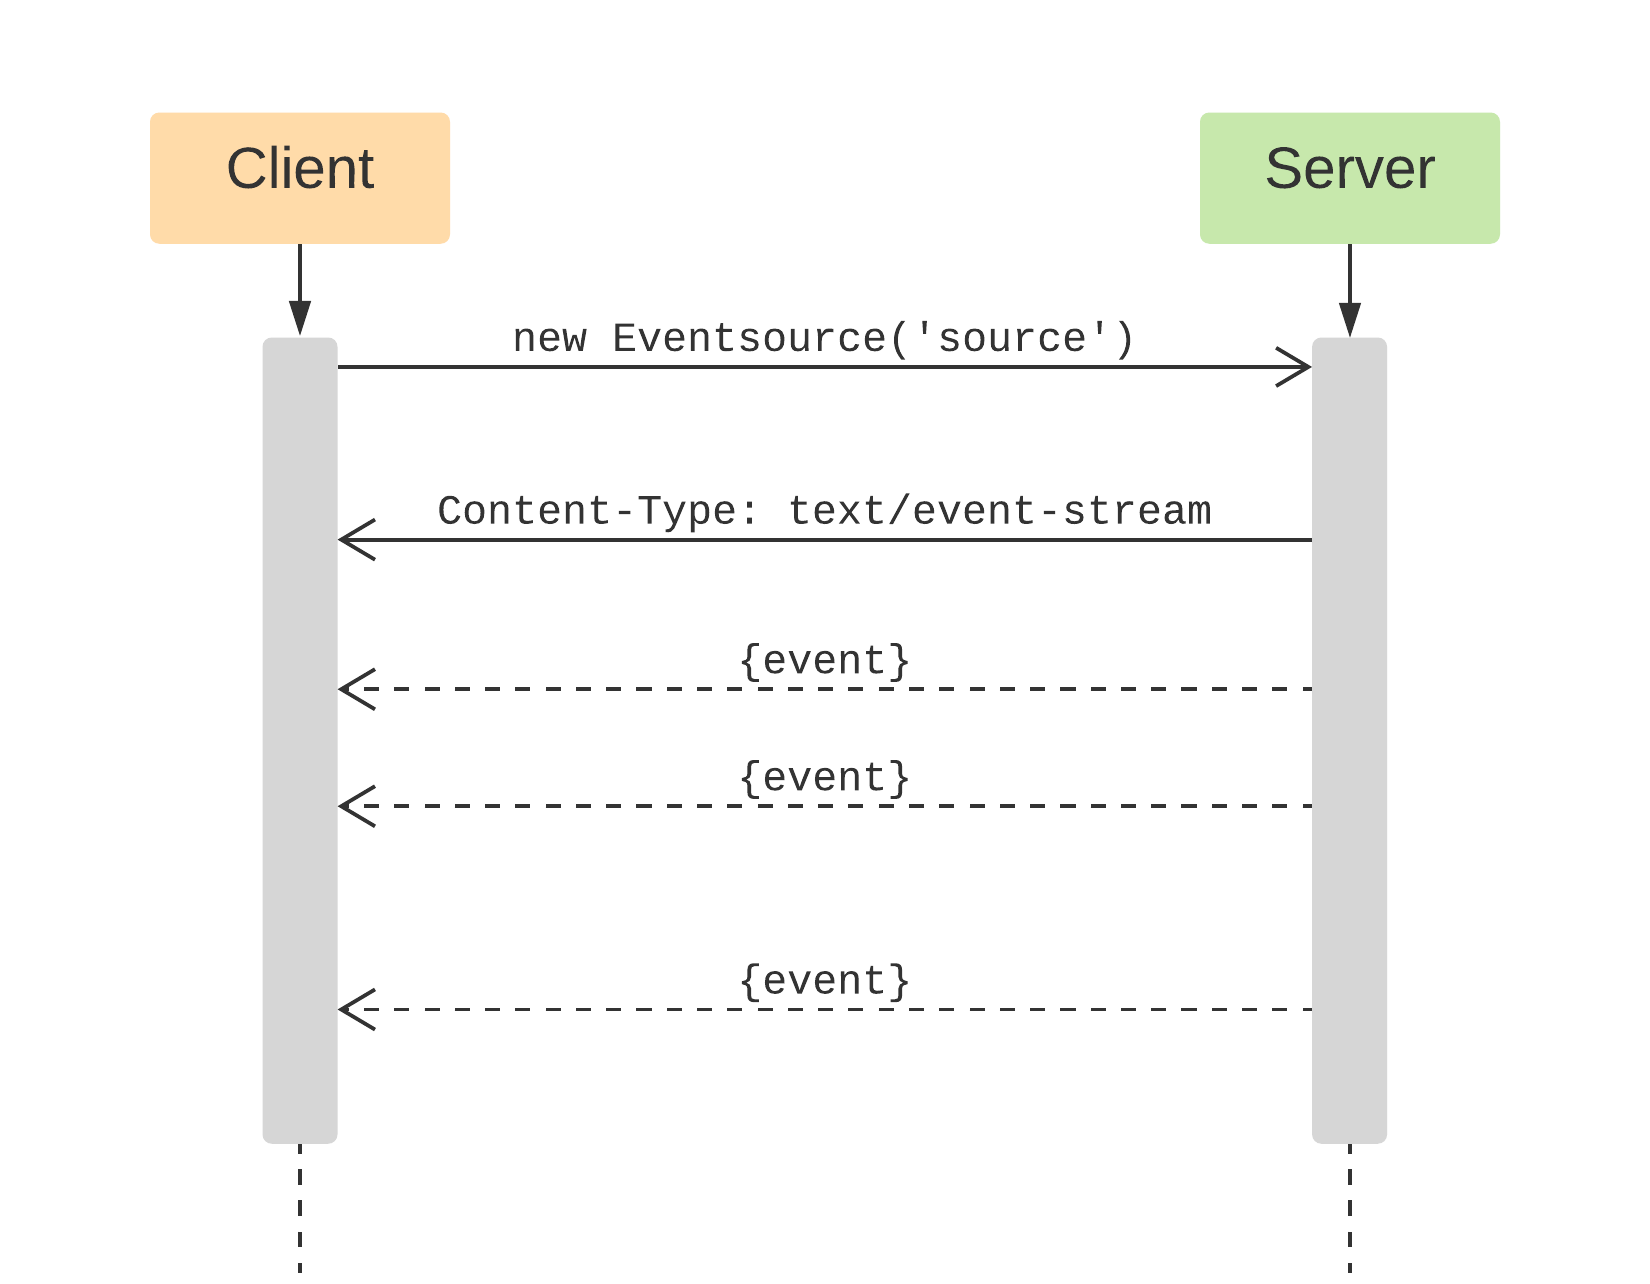
\includegraphics[width=.6\textwidth]{assets/server_sent_events.png}
\caption{Server Sent Events Flow}
\label{fig:server_sent_events}
\end{figure}

Un esempio di utilizzo di quest'API è il seguente:
\lstinputlisting[caption=Client side EventSource example]{snippets/eventsource_sample.js}

La limitazione di questa tecnologia è che una volta aperta una connessione, il client non potrà sfruttare la stessa per inviare ulteriori messaggi. Ciò significa che per rimanere in ascolto di diverse risorse in instanti differenti, sarà necessario aprire più connessioni. Se invece il server supporta HTTP/2, SSE potrà sfruttare il multiplexing offerto da HTTP/2 automaticamente.
Inoltre, al momento di questa stesura, nessuna versione di Internet Explorer e nessuna versione precedente alla 75 di Edge supportano i SSE\cite{sse_support_caniuse}.

%%%%%%%%%%%%%%%%%%%%%%%%%
		% WebSockets
%%%%%%%%%%%%%%%%%%%%%%%%%
\subsection{WebSockets}
I WebSocket sono un protocollo che permette una comunicazione full-duplex\footnote{in entrambe le direzioni e contemporaneamente} mediante una singola connessione TCP.
L'RFC 6455 afferma che WebSocket è progettato in modo da funzionare attraverso le porte HTTP 80 e 433 e di supportare proxy e intermediari HTTP, rendendolo dunque compatibile con il protocollo HTTP\cite{websockets_rfc}. Per poter essere compatibile, l'handshake tramite WebSocket fa uso dell'header \lstinline{Upgrade} di HTTP per cambiare protocollo da HTTP a WebSocket. Ciò è possibile perché entrambi i protocolli fanno parte dell'application layer nel modello OSI e dipendono da TCP.

\bigskip

Nei browser i WebSocket possono essere utilizzati mediante la \textit{WebSocket API}, anch'essa presente nell'HTML Living Standard di WHATWG.
Il flusso di comunicazione basato su WebSocket può essere espresso come segue\cite{websockets} ed illustrato in figura \ref{fig:websockets}:
\begin{enumerate}
  \item Il client tramite la chiamata API \lstinline{new WebSocket('/api/myEndpoint')} apre una nuova connessione HTTP, specificando nella richiesta gli header \lstinline{Upgrade: WebSocket} e \lstinline{Connection: Upgrade}.
  \item Il client registra le callback agli eventi \lstinline{onmessage}, \lstinline{onopen}, \lstinline{onclose} e \lstinline{onerror}.
  \item Il server risponde alla richiesta con codice \lstinline{101 Switching Protocols} e gestisce il socket aperto tramite protocollo WebSocket.
  \item Il client e il server possono finalmente scambiarsi messaggi in entrambe le direzioni.
\end{enumerate}
L'implementazione è molto simile a quella dei Server Sent Events:
\lstinputlisting[caption=Client side WebSocket example]{snippets/websocket_sample.js}

\begin{figure}[!htbp]
\centering
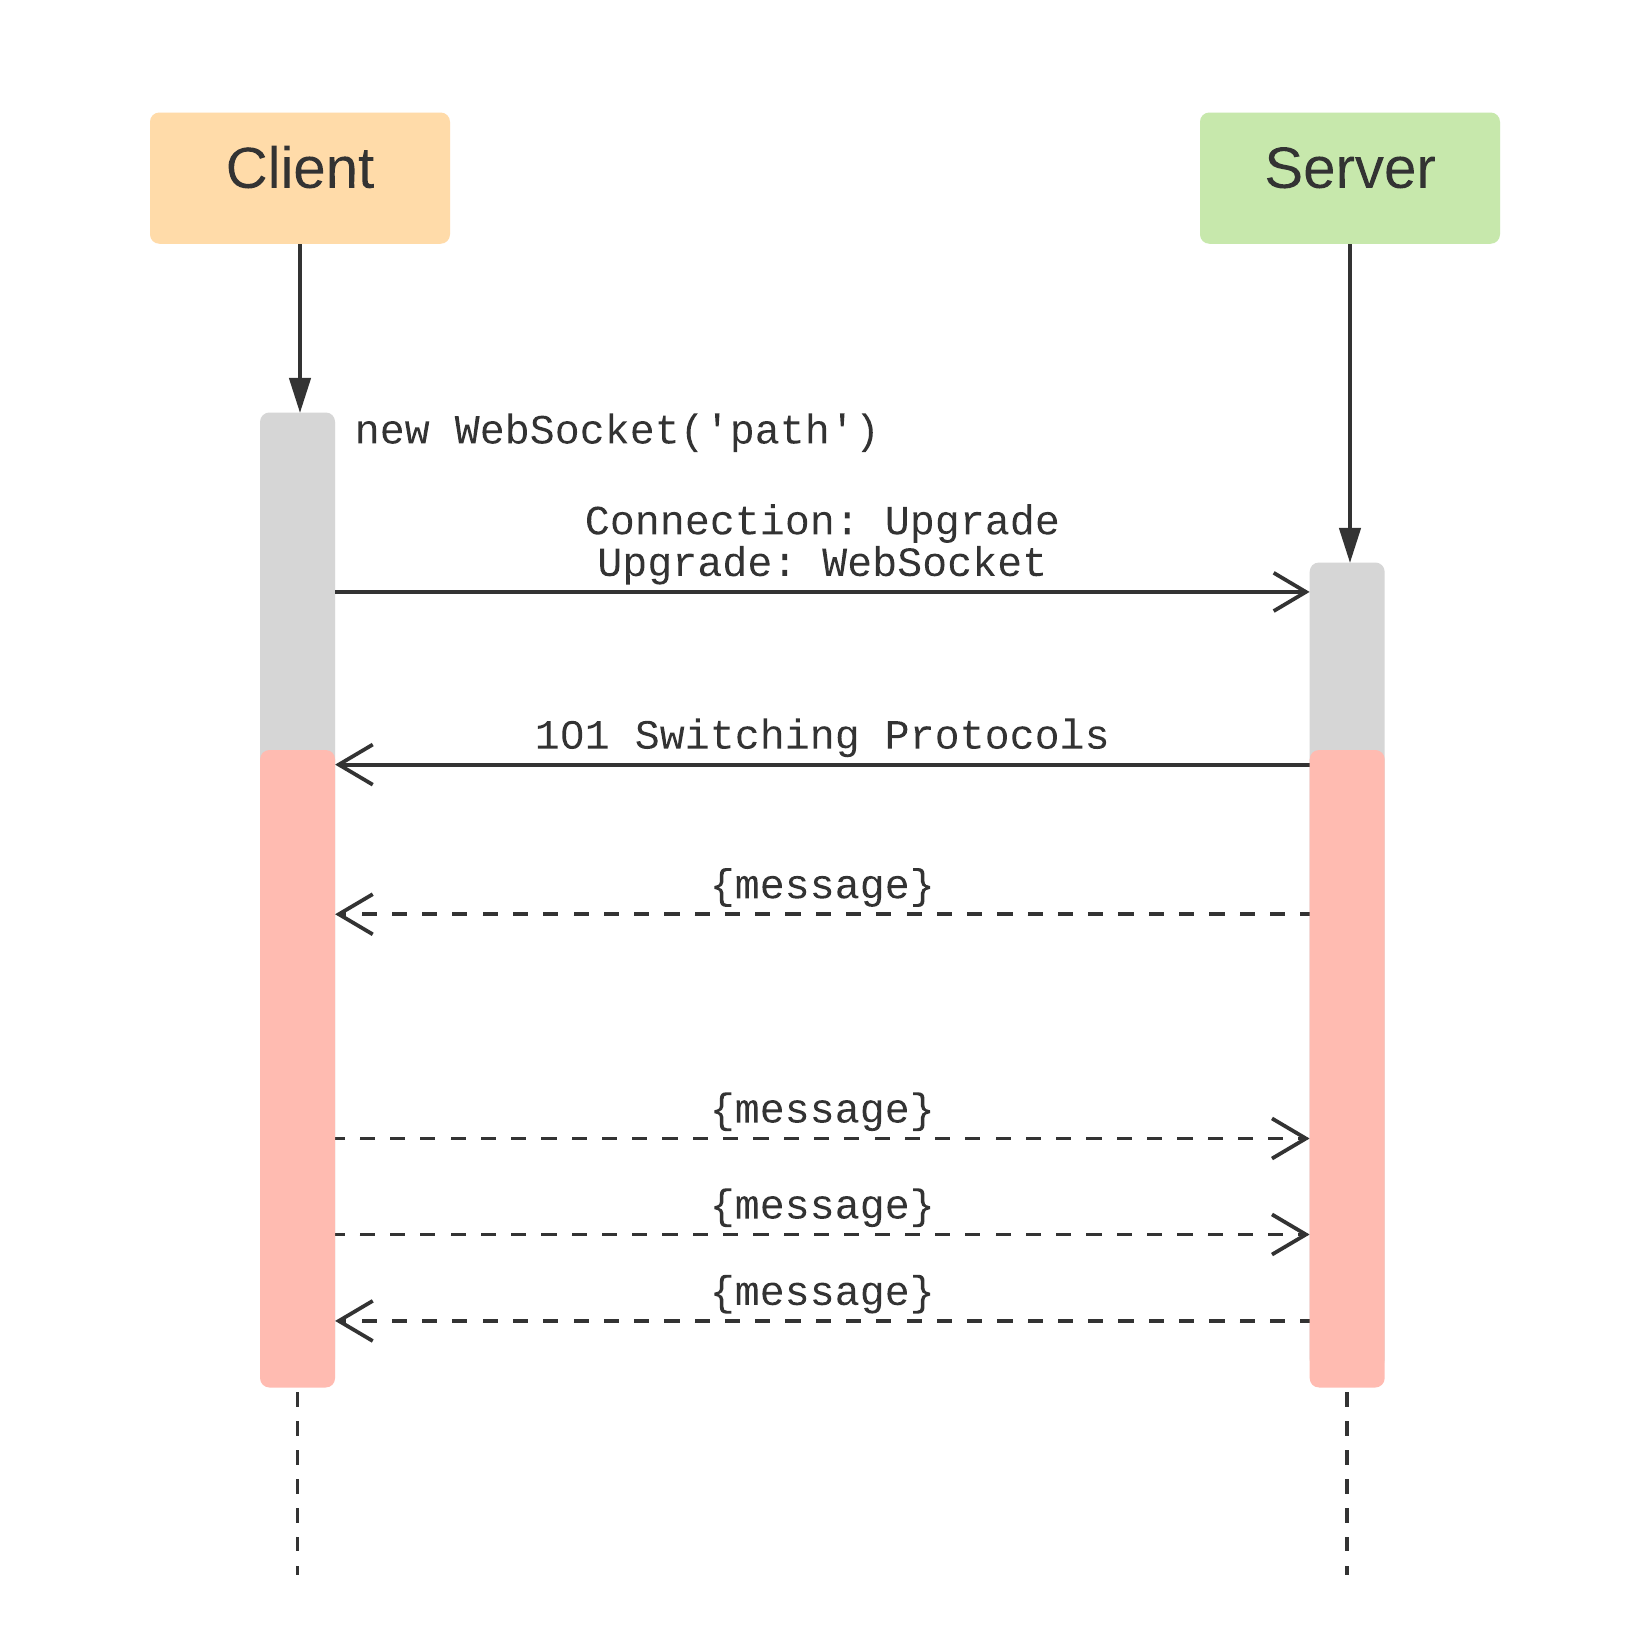
\includegraphics[width=.5\textwidth]{assets/websockets.png}
\caption{WebSockets Flow}
\label{fig:websockets}
\end{figure}
I WebSocket sono supportati da tutti i browser moderni. 
Sfortunatamente al momento della stesura non è possibile comunicare con i WebSocket tramite HTTP/2, in quanto non dispone del meccanismo di Upgrade di HTTP/1.1. Tuttavia i browser si stanno adoperando per supportare l'apertura di una comunicazione attraverso WebSocket su HTTP/2 seguendo il recente RCF 8441\cite{websockets_http2_rfc}. Ciò porterà a poter sfruttare il multiplexing offerto da HTTP/2 automaticamente anche con i WebSocket.
%%%%%%%%%%%%%%%%%%%%%%%%%%%%%%%%%%%%%%%%%%%%%%%%%%%%%%%%%%%%%%%%%%%%%%%%%%%
							% Listen JS
%%%%%%%%%%%%%%%%%%%%%%%%%%%%%%%%%%%%%%%%%%%%%%%%%%%%%%%%%%%%%%%%%%%%%%%%%%%
\chapter{Listen JS}
Il mio contributo nell'ambito dello sviluppo di web application real-time si concretizza in Listen JS, un insieme di librerie che permettono di osservare in tempo reale gli aggiornamenti ad una o più risorse.
Il progetto comprende anche un'applicazione di esempio che permette a più utenti di collaborare sull'inserimento, la modifica e la cancellazione di appuntamenti su un calendario tramite una web app.

\bigskip

Le librerie messe a disposizione sono rispettivamente \lstinline{listenjs} e \lstinline{listenjs-server}, la prima è una libreria client, utilizzabile su qualsiasi browser che supporti i WebSocket, la seconda è una libreria server utilizzabile su server sviluppati in NodeJS.
Entrambe le librerie sono volutamente framework-agnostic, cioè possono essere facilmente integrate in qualsiasi framework già esistente, sia front-end (e.g. Angular, React, VueJS...) che back-end (e.g. Express, Fastify, Koa...), e non sono opinionate rispetto ad alcun paradigma di programmazione. Utilizzando costrutti già presenti in Javascript, e non avendo dipendenze ad altre librerie, possono essere integrate in una codebase già esistente apportando pochissime modifiche.

\bigskip

Listen JS è volta a diminuire l'inerzia dell'implementazione di un'app real-time basata su WebSocket facilitandone l'utilizzo e riducendo il codice boilerplate. Inoltre fornisce una serie di funzionalità descritte nella sezione \ref{sec_features} per migliorare la gestione delle risorse, l'affidabilità e la semplicità d'utilizzo.
%%%%%%%%%%%%%%%%%%%%%%%%%
			% Struttura ad alto livello
%%%%%%%%%%%%%%%%%%%%%%%%%
\section{Struttura ad alto livello}\label{sec_struttura_alto_livello}
Le librerie utilizzano i WebSocket come layer di trasporto e astraggono la comunicazione scambiandosi dei messaggi predefiniti, ma che contengono payload definiti dall'utente.
La scelta di utilizzare i WebSocket come trasporto invece dei Server Sent Events è dovuta ai seguenti motivi:
\begin{enumerate}
\item I WebSocket sono supportati da tutti i browser moderni, a differenza dei Server Sent Events che (al momento della stesura) non sono supportati da Internet Explorer e alcune versioni di Edge.
\item Con i Server Sent Events non è possibile fare multiplexing utilizzando HTTP/1.1, in quanto non è possibile inviare messaggi successivi da client a server utilizzando la stessa connessione.
\item Poiché con i Server Sent Events non si possono inviare messaggi da client a server sulla stessa connessione, risulta difficile implementare meccanismi di ping personalizzati. È dunque complicato lato client verificare quando un server non è più raggiungibile.
\end{enumerate}
Il client può mettersi in ascolto di una o più risorse in qualsiasi istante nel tempo, e ricevere aggiornamenti in tempo reale delle risorse osservate, come in figura \ref{fig:listenjs}.
\begin{figure}[!htbp]
\centering

\includegraphics[width=.7\textwidth]{assets/listenjs.png}
\caption{ListenJS client-server interaction}
\label{fig:listenjs}
\end{figure}

\subsection{Libreria client}
La libreria client permette con una linea di codice di rimanere in ascolto di qualsiasi risorsa negli endpoint che si desidera.

\subsubsection{Installazione}
La libreria client di ListenJS può essere aggiunta ad un progetto che sfrutti un module bundler (come per esempio WebPack) tramite il package manager NPM, eseguendo il comando:
\begin{center}
\lstinline{npm install @filippovigani/listenjs}
\end{center}
per poi essere importata o tramite CommonJS o gli import dei moduli di ES6:
\begin{center}
\lstinline{const listen = require('@filippovigani/listenjs').listen}
\end{center}
oppure
\begin{center}
\lstinline|import { listen, ... } from "@filippovigani/listenjs/listen"|
\end{center}  
Alternativamente è possibile scaricare direttamente il codice sorgente\cite{listenjs_repo} e importarlo nel progetto che si desidera.

\subsubsection{Utilizzo}
Per ogni risorsa per cui si vuole essere notificati degli aggiornamenti, basterà semplicemente chiamare la funzione per ascoltare uno specifico endpoint:
\lstinputlisting[caption=Listen JS client example]{snippets/listenjsclient_sample.js}
L'URI passato come argomento della funzione, può sia essere relativo, e quindi utilizzare lo stesso dominio della pagina di origine, oppure specificare un indirizzo completo, per esempio \lstinline{differentDomain.com/api/appointments}. Questo dominio per permettere al protocollo di WebSocket di fare l'handshake, dovrà avere abilitato i CORS (Cross-Origin Resource Sharing) in quanto la risorsa è su un'origine differente.

\subsection{Libreria server}
La libreria server permette di inizializzare un server che supporti i WebSocket e gestisce i client in ascolto sulle varie risorse, permettendo di notificare tutti i client in ascolto su una specifica risorsa. 
\subsubsection{Installazione}
Per aggiungere la libreria server di ListenJS ad un progetto NodeJS è sufficiente eseguire il comando:
\begin{center}
\lstinline{npm install @filippovigani/listenjs-server}
\end{center}
e per poterla utilizzare basta importarla come tutti i moduli di NodeJS
\begin{center}
\lstinline{const listen = require('@filippovigani/listenjs-server')}
\end{center}
Come per la parte client, è in alternativa possibile scaricare il codice sorgente\cite{listenjs_server_repo} e importarlo manualmente nel progetto.

\subsubsection{Utilizzo}
In fase di inizializzazione del server è necessario fare il binding di un server HTTP di NodeJS già esistente con ListenJS, per poter inizializzare connessioni tramite WebSocket. Ciò si può fare chiamando la funzione \lstinline{setup} come segue: 
\lstinputlisting[caption=Listen JS server setup example]{snippets/listenjsserver_sample.js}
In caso fossero utilizzati framework per il routing degli endpoint, è sempre possibile reperire l'istanza del server HTTP sottostante per poter inizializzare ListenJS. Per esempio, utilizzando Fastify, ListenJS verrà inizializzato in questo modo:
\lstinputlisting[caption=Listen JS Fastify setup example]{snippets/listenjsserver_fastify_sample.js}
Per qualsiasi altro framework si può trovare nella documentazione come reperire il server HTTP.

\bigskip

Una volta inizializzato, è possibile notificare i client che sono in ascolto di una risorsa tramite la funzione \lstinline{notify}. Per esempio, in un endpoint POST, il codice per notificare tutti i client in ascolto su una risorsa è il seguente:
\lstinputlisting[caption=Listen JS server notify example]{snippets/listenjsserver_notify_sample.js}

La libreria si occuperà di inviare un messaggio contentente il nuovo payload a tutti e soli i client in ascolto. Se non ci fosse nessun client in ascolto su quella specifica risorsa, la chiamata non avrà alcun effetto.

%%%%%%%%%%%%%%%%%%%%%%%%%
			% Features
%%%%%%%%%%%%%%%%%%%%%%%%%
\section{Features}\label{sec_features}
Oltre a semplificare la comunicazione dell'aggiornamento delle varie risorse in ascolto dai client, ListenJS implementa una serie di funzionalità per semplificare la vita allo sviluppatore, e permettere di adempire al Single Responsibility Principle\cite{single_responsibility_principle} nell'applicazione real-time che utilizza questo sistema di comunicazione.
\subsection{Disconnection detection}
L'evento \lstinline{onclose} fornito dai WebSocket viene lanciato solo nel caso in cui il socket venga chiuso esplicitamente o dal client o dal server tramite l'handshake di chiusura specificato nell'RFC 6455. Tuttavia, in caso di problemi di network, la chiusura del socket non verrà notificata, né dal client né dal server. In aggiunta, i messaggi scambiati in caso di pessime condizioni di network verranno lasciate in sospese.

\bigskip

Per ovviare a questo problema ListenJS implementa un sistema di heartbeat (aka ping-pong), che fa si che il client invii periodicamente dei messaggi di ping, aspettandosi un messaggio di pong dal server entro un certo timeout. Se non dovesse riceverlo, allora considererà il socket come chiuso, provando ad iniziare l'handshake di chiusura tramite la chiamata alla WebSocket API. Di contro, il server si aspetterà di ricevere un messaggio di ping ogni intervallo prestabilito. Se non dovesse succedere, allora si aspetterà di non avere più connettività con il client, chiudendo il socket.
\subsection{Reconnection}
I WebSocket non permettono di riaprire un socket precedentemente chiuso. Ciò comporta che in caso di disconnessione dovuta a delle condizioni di network non ottimali, non sia possibile riutilizzare lo stesso socket per mantenere la sessione precedente attiva.

\bigskip

ListenJS fornisce un sistema di riconnessione aprendo un nuovo WebSocket, ma mantenendo le informazioni di uno specifico client come se la sessione precedente fosse ripristinata. Ciò significa che il client non dovrà preoccuparsi di rimettersi in ascolto delle risorse precedentemente specificate, ma sarà tutto gestito dalla libreria.

\subsection{Multiplexing}
Un'implementazione naïve per rimanere in ascolto di alcune risorse potrebbe essere quella di aprire un WebSocket per ogni risorsa che si vuole osservare, specificando l'URL della risorsa nel pacchetto di handshake. Per esempio, se volessimo rimanere in ascolto di due risorse \lstinline{foo} e \lstinline{bar}, potremmo aprire due WebSocket chiamando \lstinline{new WebSocket('ws://myDomain.com/api/foo')} e \lstinline{new WebSocket('ws://myDomain.com/api/bar')}. Tuttavia così facendo si aprirebbero due connessioni separate, che non è ideale per due motivazioni:
\begin{itemize}
\item I browser limitano il numero di connessioni HTTP contemporanee su uno stesso dominio\cite{http11_rfc}. La maggior parte dei browser moderni consentono un massimo di sei connessioni per dominio.
\item Per aprire un WebSocket c'è un ritardo dovuto all'handshake specificato dal protocollo, che potrebbe essere evitato utilizzando lo stesso socket.
\end{itemize}

\bigskip

Per evitare questi problemi, ListenJS sfrutta intelligentemente le connessioni attive. Dunque, se non esiste un socket aperto per uno specifico dominio, allora ne aprirà uno, altrimenti riutilizzerà lo stesso socket per scambiare ulteriori messaggi. Per fare un parallelismo con l'esempio precedente, se con la libreria client si decidesse di osservare prima \lstinline{foo} e poi \lstinline{bar} sullo stesso dominio, prima verrebbe aperto un socket per il dominio, mentre successivamente verrebbe riutilizzato il socket già aperto per comunicare l'intenzione di mettersi in ascolto su \lstinline{bar}.
In aggiunta, se nel ciclo di vita dell'applicazione non ci fosse più nessuna risorsa osservata su uno stesso dominio, ListenJS si occuperà di chiudere il socket per liberare le risorse utilizzate.

%%%%%%%%%%%%%%%%%%%%%%%%%
			% Struttura a basso livello
%%%%%%%%%%%%%%%%%%%%%%%%%
\section{Struttura a basso livello}\label{sec_struttura_basso_livello}
Abbiamo visto ad alto livello cosa offre ListenJS e in generale come queste funzionalità sono utili nello sviluppo di applicazioni real-time. Possiamo ora andare più a fondo nel funzionamento specifico, in modo da avere le basi per estendere e potenzialmente migliorare questi comportamenti.

\subsection{Message channel}
Il funzionamento del sistema si basa sullo scambio dei messaggi che hanno una struttura ben specifica, e conosciuta sia dal client che dal server. Ogni messaggio può essere un \textit{Control Message} o un \textit{Payload Message}, e sono dei messaggi testuali serializzati in JSON come segue:
\lstinputlisting[caption=Listen JS Message Contract]{snippets/listenjs_message.json}
Più altri valori specifici di una certa azione. In particolare, \lstinline{<ACTION>} è una stringa che specifica il tipo di messaggio di controllo (o di payload), e può assumere i seguenti valori:
\begin{itemize}
\item Da client a server:
  \begin{itemize}
  \item \lstinline{HANDSHAKE}: Specifica un messaggio di controllo per inizializzare un nuova nuova connessione con un client. Facoltativamente può essere specificato un \lstinline{clientId} come campo extra per ripristinare una sessione di uno specifico client. Se il server non riceve nessun messaggio di handshake entro un timeout specificato (default: 10000 ms) da quando un socket viene aperto, chiude automaticamente la connessione.
  \item \lstinline{SUBSCRIBE}: Specifica che il client desidera mettersi in ascolto dell'endpoint specificato con il campo \lstinline{path}, tramite un observer gestito dal client con \lstinline{observerId}.
  \item \lstinline{UNSUBSCRIBE}: Specifica che il client non desidera più ricevere notifiche di aggiornamenti dell'endpoint specificato con il campo \lstinline{path}.
  \item \lstinline{HEARTBEAT}: Invia un messaggio di ping al server per verificare che sia ancora raggiungibile.
  \end{itemize}
\item Da server a client:
  \begin{itemize}
  \item \lstinline{HANDSHAKE_ACK}: Risponde ad un messaggio di handshake, chiudendo la procedura di riconoscimento del client. Se un \lstinline{clientId} è specificato come campo, allora verrà ripristinato quel client, recuperando le informazioni sulle risorse che sta ascoltando. Altrimenti, genererà un \lstinline{clientId} univoco come UUID (e.g. \lstinline{B16B00B5-81F6-A420-81F6-008C3285ADB9}).
  \item \lstinline{SUBSCRIBE_ACK}: Conferma al client che la sottoscrizione alla risorsa in ascolto da \lstinline{observerId} è avvenuta con successo.
  \item \lstinline{UNSUBSCRIBE_ACK}: Conferma al client l'avvenuta rimozione delle sottoscrizioni alla risorsa specificata dal suo \lstinline{path}.
  \item \lstinline{HEARTBEAT_ACK}: Invia un messaggio di pong al client in risposta ad un ping.
  \item \lstinline{UPDATE}: Invia un messaggio di payload al client, specificandone il contenuto nel campo \lstinline{body} e la risorsa di riferimento nel campo \lstinline{path}.
  \end{itemize}
\end{itemize}

Questa è la definizione formale del canale di comunicazione tra libreria client e libreria server. Per quanto riguarda i dettagli implementativi specifici dell'una o dell'altra, risulta più semplice andare ad analizzare singolarmente come le feature siano state implementate.

\subsection{Observer pattern across the stack}
La Gang of Four definisce l'observer pattern\cite{observer} come un behavioral pattern che prevede che un certo numero di observer siano notificati quando un subject subisce un cambiamento di stato. Questo tipo di pattern è largamente utilizzato nel design di interfacce grafiche, dove si vuole ridurre al minimo il coupling tra le classi per non renderle meno riutilizzabili. Questo però non significa che possa essere utilizzato in ambiti al di fuori dello sviluppo di UI.

\bigskip

Nel nostro caso, l'observer pattern viene inteso come publish/subscribe, e funziona attraverso i differenti layer di comunicazione. Ciò significa che viene in primo luogo applicato ad un livello di astrazione più alto, dove gli observer sono i vari client, e il subject è il server.

Inoltre, lo stesso pattern viene applicato nella gestione del client, dove si hanno diversi observer che stanno in ascolto di una specifica risorsa. Quando un messaggio di payload viene ricevuto da un \textit{manager} del client, questo viene inoltrato agli observer corretti che sono in ascolto su una risorsa.

In ListenJS il manager è un'istanza che gestisce la connessione ad uno specifico dominio. Ogni manager tiene in memoria una lista di observer. Quando si effettua la chiamata \lstinline{listen(path)}, viene creato un nuovo observer per il path specificato, ed aggiunto al manager.

Un observer è descritto dalle seguenti proprietà:
\begin{itemize}
\item \lstinline{id}: Identifica l'observer univocamente
\item \lstinline{path}: Indica il path che l'observer desidera osservare
\item \lstinline{status}: Indica lo stato dell'observer, che può essere:
  \begin{itemize}
  \item \lstinline{WAITING_HANDSHAKE}: L'observer è stato appena inizializzato e sta attendendo che un handshake sia completato per potersi sottoscrivere
  \item \lstinline{SUBSCRIBING}: Il manager ha inviato la richiesta di osservare l'endpoint, ma sta attendendo di ricevere una conferma
  \item \lstinline{UNSUBSCRIBING}: Il manager ha inviato la richiesta di non osservare più l'endpoint
  \item \lstinline{LISTENING}: L'observer sta correttamente ascoltando gli aggiornamenti ad una risorsa
  \item \lstinline{ERROR}: Un errore imprevisto
  \end{itemize}
\end{itemize}

Come l'observer, anche il manager mantiene uno stato interno che indica la fase della connessione. Lo stato del manager è legato agli eventi ricevuti dal socket, ma è più preciso sulla fase di connessione:
\begin{itemize}
\item \lstinline{IDLE}: Manager appena inizializzato
\item \lstinline{CONNECTING}: Il socket è in fase di connessione
\item \lstinline{HANDSHAKING}: Il socket è connesso ma il manager non ha ancora finito la fase di handshake
\item \lstinline{CONNECTED}: Il socket è connesso e l'handshake è stato eseguito correttamente
\item \lstinline{DISCONNECTED}: Il socket è disconnesso
\item \lstinline{RECONNECTING}: Il socket è in fase di connessione dopo che un altro socket è stato chiuso
\item \lstinline{ERROR}: Un errore imprevisto
\end{itemize}

Il manager gestisce sia gli observer, che il socket. 
In particolare, quando un nuovo observer viene aggiunto al manager, esso utilizza il proprio stato interno per capire quando sia opportuno inviare i messaggi di controllo. Per esempio, se viene aggiunto un nuovo observer, ma lo stato del manager è \lstinline{CONNECTING} o \lstinline{HANDSHAKING}, allora dovrà mettersi in attesa che il proprio stato sia propriamente \lstinline{CONNECTED}. Una volta \lstinline{CONNECTED} (o nel caso lo fosse già in fase di aggiunta), potrà procedere ad inviare tramite il socket i messaggi di controllo per fare il \lstinline{SUBSCRIBE} del \lstinline{path} specificato.
Inoltre, il manager si occupa di aprire un nuovo socket appena un nuovo observer viene aggiunto. Quando invece vengono rimossi tutti gli observer per lo stesso manager, allora si occuperà di chiudere il socket attuale.


\subsection{Implementazione multiplexing}

\subsection{Implementazione disconnection detection}
contratto ping su handshake
ping/keep alive
\subsection{Implementazione reconnection}
backoff


%%%%%%%%%%%%%%%%%%%%%%%%%
			% Applicazione di esempio
%%%%%%%%%%%%%%%%%%%%%%%%%
\section{Applicazione di esempio}\label{sec_applicazioneesempio}
CORS
%%%%%%%%%%%%%%%%%%%%%%%%%%%%%%%%%%%%%%%%%%%%%%%%%%%%%%%%%%%%%%%%%%%%%%%%%%%
							% Valutazione
%%%%%%%%%%%%%%%%%%%%%%%%%%%%%%%%%%%%%%%%%%%%%%%%%%%%%%%%%%%%%%%%%%%%%%%%%%%
\chapter{Valutazione}

%%%%%%%%%%%%%%%%%%%%%%%%%
			% Confronto tra XHR polling e WebSocket
%%%%%%%%%%%%%%%%%%%%%%%%%
\section{Confronto tra XHR polling e websockets}\label{sec_confrontopollingwebsockets}

\subsection{Responsiveness}

\subsection{Traffico dati}

\subsection{User experience}
Tradeoff

%%%%%%%%%%%%%%%%%%%%%%%%%
			% Valore aggiunto di Listen JS
%%%%%%%%%%%%%%%%%%%%%%%%%
\section{Valore aggiunto di Listen JS}\label{sec_valorelistenjs}

\subsection{Utilizzo risorse e limitazioni browser}
Limite socket aperti contemporaneamente

\subsection{Immediatezza integrazione da parte di sviluppatori}

\subsection{Architettura}
Separation of Concerns

%%%%%%%%%%%%%%%%%%%%%%%%%%%%%%%%%%%%%%%%%%%%%%%%%%%%%%%%%%%%%%%%%%%%%%%%%%%
						% Conclusioni
%%%%%%%%%%%%%%%%%%%%%%%%%%%%%%%%%%%%%%%%%%%%%%%%%%%%%%%%%%%%%%%%%%%%%%%%%%%
\clearpage{\pagestyle{empty}\cleardoublepage}
\chapter*{Conclusioni}
%\rhead[\fancyplain{}{\bfseries
%Conclusioni}]{\fancyplain{}{\bfseries\thepage}}
%\lhead[\fancyplain{}{\bfseries\thepage}]{\fancyplain{}{\bfseries
%Conclusioni}}
\addcontentsline{toc}{chapter}{Conclusioni}

%%%%%%%%%%%%%%%%%%%%%%%%%%%%%%%%%%%%%%%%%%%%%%%%%%%%%%%%%%%%%%%%%%%%%%%%%%%
							% Sviluppi futuri
%%%%%%%%%%%%%%%%%%%%%%%%%%%%%%%%%%%%%%%%%%%%%%%%%%%%%%%%%%%%%%%%%%%%%%%%%%%
\chapter{Sviluppi futuri}
SSL
delta messaging
message queue
%%%%%%%%%%%%%%%%%%%%%%%%%%%%%%%%%%%%%%%%%%%%%%%%%%%%%%%%%%%%%%%%%%%%%%%%%%%
							% Bibliografia
%%%%%%%%%%%%%%%%%%%%%%%%%%%%%%%%%%%%%%%%%%%%%%%%%%%%%%%%%%%%%%%%%%%%%%%%%%%
\clearpage{\pagestyle{empty}\cleardoublepage}

%\rhead[\fancyplain{}{\bfseries
%Bibliografia}]{\fancyplain{}{\bfseries\thepage}}
%\lhead[\fancyplain{}{\bfseries\thepage}]{\fancyplain{}{\bfseries
%Bibliografia}}

\bibliographystyle{unsrt}
\bibliography{bibliografia}
\addcontentsline{toc}{chapter}{Bibliografia}

\end{document}
